%!TEX root = ../USthesis_Masters.tex
\chapter{Introduction}
\label{chp:Intro}

Bitcoin \cite{Nakamoto2008} is a peer-to-peer decentralised digital payment mechanism that was introduced in a paper published by a person or group called Satoshi Nakamoto in 2008. Bitcoin aims to be an alternative to centralised online payment mechanisms like credit cards and PayPal \cite{PayPal2015}. 

This thesis focuses on testing the viability of Bitcoin as payment mechanism on social media platforms, specifically on a mobile platfom. We want to investigate the practical viability of using Bitcoin to make small payments at a small or zero fee. One of our main goals is to compare Bitcoin with current payment mechanisms in terms of transaction fees. Bitcoin fees are not mandatory in all cases. When fees are required, the value of the fee is not fixed \cite{bitcoinwiki}. We want to investigate how these fees work and practically confirm that we can make payments with very small transaction fees.

To test the viability, we will design a Bitcoin payment framework that allows third-party developers to incorporate Bitcoin payments in their applications without having to understand the low-level details of Bitcoin and without running any Bitcoin software. 

We will also design and build a Bitcoin wallet application that will run on the social media platform to make payments directly from the application. We will also create a use-case application that simulates a third-party developer that will use the payment framework to receive Bitcoin payments.




%%%%%%%%%%%%%%%%%%%%%%%%%%%%%%%%%%%%%%%%%%%%%%%%%%%%%%%%%%%%%%%%%%%%%%%
\section{Background}

Making payments on a mobile social media platform has been done in several different ways in the past. One of the biggest challenges to overcome is that many users do not have a credit card. For many social media platforms, this is especially true since the target audience of the platform is teenagers. 

With Apple's in-app purchases \cite{apple}, credit card details have to be loaded in only once. A parent can load a credit card for a child and let the child use it, but this can lead to problems of unregulated spending.

Another common method of payment is using mobile airtime as payment. Airtime is easy to use, but the cost to the merchant is high.

The last payment method we look at is a voucher based system, like Apple's Gift Cards. Vouchers are similar to airtime as payment, but the voucher credit can only be used on the specific platform. Vouchers, like airtime, can be purchased at supermarkets. However, since the voucher is issued by the company with only the supermarket as middle-man, it follows that the loss that the company makes on overhead is less than with airtime.

We would like to test the viability of Bitcoin as an alternative to these methods of payment, especially to take advantage of Bitcoin's low transaction fees.

Bitcoin transactions can be processed without any transaction fee \cite{bitcoinwiki}, but a small fee may be required for transactions that do not meet certain criteria discussed in chapter \ref{chp:literature_study}.

%that use a lot of unspent outputs and cause a larger transaction. A large transaction in Bitcoin refers to the bytes that the transaction uses and not the value of the Bitcoin. A small fee can also be added to speed up the processing time of the transaction. There are criticisms that say that the low price of transaction fees are unsustainable and will likely increase in the future \cite{Ka2014}.



\section{Related Work}

To compare Bitcoin as a payment method on a social media platform, we must look at existing payment methods and their advantages and disadvantages. 

\subsection{Credit and Debit Cards}

\begin{table}
	\begin{center}
		\caption{Table of preferred online method of payment \cite{tsys}.} 
		\begin{tabular}	{ | c | c | c |}
		\hline
		Credit Card & Debit Card & PayPal \\ \hline
		48\% & 30\% & 12\% \\ \hline
	 
	   % \label{fig:htaccess_file}
		\end{tabular}
		
		\label{tbl:preferred_payment}
	\end{center}
\end{table}

According to an international study done in 2014 \cite{tsys}, 48\% of people prefer to make online payments with credit cards and 30\% prefer debit cards, with 12\% preferring PayPal with the remaining 10\% using unspecified payment platforms. It is clear from these statistics that card payment methods largely dominate the online payments market. 

%\subsubsection{Advantages}

Credit card payments are easy to make and are processed quickly. The costs of transactions are very difficult to determine, since they differ from bank to bank, the merchant and the user's specific credit card package. However, credit card payments can be inexpensive, since they usually have a small fixed and percentage fee per payment that is paid by the merchant. Since credit cards are backed by a trusted third party, they are able to provide mediation. They can also provide insurance against fraud. 

%\subsubsection{Disadvantages}

According to a survey done in 2014, a quarter of adults do not have bank accounts\cite{finmark}. This makes it difficult for them to purchase anything online. Furthermore, there are prerequisites to getting a credit card, like minimum income. Credit cards also usually have a fixed monthly fee.

Using a credit card is not anonymous, since the user has to enter the card number for each payment. Every payment made by the user is traceable by the credit card company. This gives the credit card company the ability to track and profile users based on their spending\cite{visa}.

Even though credit cards have small transaction fees, they still have a small fixed fee. This is an issue when payments are very small. For example, the company PayFast \cite{PayFast} charges a fixed R2 plus 3.9\% of the payment as a fee. Therefore, when a user wants to make a R5 payment, the merchant will only receive R5 - R2 - R5 $\times$ 3.9\% = R2.81. 


\subsection{Airtime Payment}

A popular mobile messaging application, Mxit, uses airtime payments with its Mxit Moola \cite{Mxit} virtual currency. They use a system where a user sends an SMS to a specific number to make a payment. For example with Mxit Moola, a user will send an SMS costing R3 of their airtime and receive 300 Moola. This is very convenient for the user - however, it is not very profitable for the company.

\begin{table}
	\begin{center}
		\caption{Table of SMS payment payouts from bulksms.com \cite{bulksms.com}.} 
		\begin{tabular}	{ | c | c | c | c | c |}
		\hline
		\textbf{SMS Cost} & \textbf{Vodacom} &\textbf{MTN} & \textbf{Cell C} & \textbf{8ta} \\ \hline
		\textbf{R1.00} &	R0.07 &	R0.06 &	R0.09 &	R0.04 \\ \hline 
		\textbf{R1.50} &	R0.44 &	R0.31 &	R0.37 &	R0.27 \\ \hline
		\textbf{R2.00} &	R0.81 &	R0.56 &	R0.66 &	R0.52 \\ \hline
		\textbf{R3.00} &	R1.55 &	R1.08 &	R1.24 &	R0.99 \\ \hline
		\textbf{R5.00} &	R3.03 &	R2.11 &	R2.40 &	R2.06 \\ \hline
		\textbf{R7.50} &	R4.88 &	R3.39 &	R3.84 &	R3.31 \\ \hline
		\textbf{R10.00} & R6.73 & R5.10 & R5.29 & R4.57 \\ \hline
		\textbf{R15.00} & R10.43 & R7.24 & R8.18 & R7.07 \\ \hline
		\textbf{R20.00} & R14.13 & R9.81 & R11.14 & R9.58 \\ \hline
		\textbf{R25.00} & R17.83 & R10.91 & R13.96 & R12.10 \\ \hline
		\textbf{R30.00} & R21.53 & R14.40 &	R16.85 & R14.60 \\ \hline
	 
	   % \label{fig:htaccess_file}
		\end{tabular}
		
		\label{tbl:sms_prices}
	\end{center}
\end{table}

\begin{figure}
  \centering
   \caption{Graph showing payout percentages that a merchant receives for SMS payments.} 
    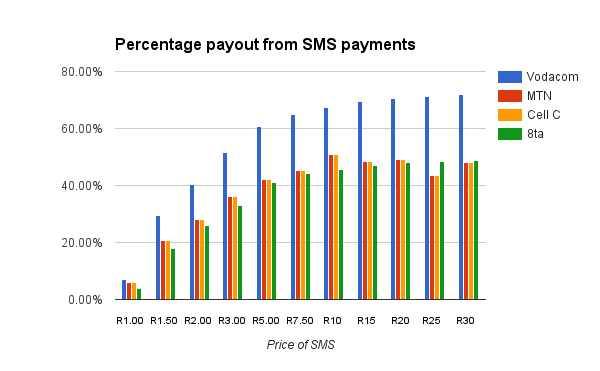
\includegraphics[width=\textwidth]{figs/sms_percentage.png}
  
   \label{fig:sms_percentage}
\end{figure}

From table \ref{tbl:sms_prices} and figure \ref{fig:sms_percentage} we can see that the company itself gets a very small percentage of the payment. This is especially true for payments less than R5, where the average payout percentage is less than 50\%. Even the highest SMS value at the network with the highest payout only has a payout of 71.77\%.

%\subsubsection{Advantages of Airtime}

The airtime model works very well, because it allows teenagers to use it with their existing airtime quotas without requiring their parents' credit card details. Airtime is also very easily accessible, since it can be bought with cash at most supermarkets among other methods. 

%\subsubsection{Disadvantages of Airtime}

Airtime as payment only has one big disadvantage - the very high transaction fee paid by the merchant. 


\subsection{Vouchers}

Vouchers are very similar to airtime in regards to accessibility. A physical voucher can usually be bought at a supermarket, where a code is sold to the user. This code is then entered by the user on the service provided by the company that provides the voucher, where the user will then receive the amount of the voucher as credit. For mobile purchases, Apple's Gift Cards are a very good example of vouchers in practice. The gift cards can be used in all the same Apple-related online stores that credit cards are used. This allows users to effectively buy online virtual goods using cash.

% \subsubsection{Advantages of Vouchers}

Vouchers are easily accessible and are purchasable using cash. They are comparable to the airtime payment model, but they provide more control to the merchant. Vouchers also enable users to budget their spending, something that is ideal for teenagers and children.

% \subsubsection{Disadvantages of Vouchers}

Vouchers can only be used at the online merchant that they are bought for. Therefore, if a person wants to pay at different online merchants, they will need to buy a voucher for each of the merchants. 

Physical vouchers that are sold at stores are physical items that have to be manufactured and distributed across the world. This adds to the overhead cost, and it is also possible for vouchers to be sold out in certain places.

\section{Objectives}

Our objective is to test the viability of Bitcoin as a payment mechanism on a social media platform. The platform chosen is a text-messaging social media application called WeChat.

We want to test how Bitcoin compares to alternative payment mechanisms on the following criteria:

\begin{itemize}
	\item{Transaction fees}
	\item{Ease of use}
	\item{Versatility}
\end{itemize}

To test the viability of Bitcoin, we will implement a Bitcoin payment system that runs on WeChat. This payment system should resemble a Bitcoin wallet application that allows users to send and receive Bitcoin. 

The Bitcoin wallet's main objective will be to make payments within the WeChat application. Therefore, our main objective is to design the payment framework that other applications within WeChat will use to request and receive payments. This payment framework should also be able to confirm that a payment has been made. 

We also want to test the practical limitations of making small Bitcoin transactions with low transaction fees. We want to investigate the effect of lowering the transaction fees and find a practical lower bound of transaction fees.

To implement our Bitcoin payments framework and wallet application, we will design a use-case application that also runs on WeChat. We will design and implement an application where gamebooks are sold and read. This application should present the user with a list of books that can be bought. The user should then be able to pay for the book by using our wallet application or any Bitcoin wallet application. If the payment is successful, the user should be able to read the gamebook on their phone.

Therefore, the objective is to be able to receive Bitcoin payments on a social media platform with smaller transaction fees than other payment systems.


% In granular or particle flow simulations with Discrete Element Method (DEM),
% the mechanical behavior of a system of particles are simulated. The basic
% building blocks of DEM are finite sized particles and walls. It is generally
% classified into two basically different approaches.

% The first is the ``hard sphere'', event-driven method
% \citep[e.g.][]{Luding-1994, Luding-2004}, where particles are assumed to be
% perfectly rigid and they follow an undisturbed motion until a collision
% occurs. Due to the rigidity of the interaction, the collisions occur
% instantaneously with accompanying momentum transfer. It is mainly used for
% collisional, dissipative granular gases.

% The second is the so-called ``soft particle'' molecular dynamics pioneered by
% \citet{Cundall-1979}, where the particles are allowed to overlap or penetrate
% each other. Constrains on the physical space that a particle can occupy at a
% specific time is included with contact or penalty forces related to the
% amount of overlap and contact velocity between particles or between particles
% and walls. The motion of the system is modelled by the integration of
% Newton-Euler equations for motion of every individual particle.
